
\documentclass[11pt,a4paper]{scrartcl}
\usepackage[utf8]{inputenc}
\usepackage[english]{babel}
\usepackage{microtype}
\usepackage{amsmath}
\usepackage{mathtools}
%\usepackage[leqno]{amsmath}
\usepackage{amsfonts}
\usepackage{amssymb}
\usepackage{graphicx}
\usepackage{indentfirst}
\usepackage{fancyvrb}
%\usepackage{subfigure}
\usepackage{caption}
\usepackage{subcaption}
\usepackage{enumitem}
\usepackage{booktabs}
\usepackage{algorithm}
\usepackage{algpseudocode}
\usepackage[onehalfspacing]{setspace}
\usepackage[hidelinks]{hyperref}
\usepackage{listings}
\usepackage{xcolor}
\usepackage{fancyhdr}
\pagestyle{fancy}
\fancyhf{}
\fancyhead[R]{\thepage}

\usepackage{amsmath}
\usepackage{nccmath}
\newenvironment{mpmatrix}{\begin{medsize}\begin{pmatrix}}%
{\end{pmatrix}\end{medsize}}%

\date{}
\title{STDP-based spiking deep convolutional neural networks for object recognition}
\begin{document}

\begin{titlepage}
\begin{center}
	
\includegraphics[scale=0.8]{images/SapienzaLogo} \\
	\vspace{3em}
	{\large \textsc{Facoltà di  Ingegneria dell'informazione, Informatica e Statistica}} \\
	\vspace{2em}
	{\large \textsc{Neural Networks}} \\
	\doublespacing
	\vspace{5em}
	{\Large \textbf{STDP-based spiking deep convolutional neural networks for object recognition}}
\end{center}

\vskip 2cm
\begin{center}
\begin{tabular}{c c c c c c c c}
	Supervisor & & & & & & & Students \\[0.2cm]
	\large{Simone Scardapane} & & & & & & & \large{Edoardo Ghini}\\[0.2cm]
	\large{} & & & & & & & \large{Gianluca Cerilli}\\
	\end{tabular}
\end{center}

\vskip 1.5cm
\begin{center}
	{\normalsize Academic Year 2017/2018}
\end{center}
\end{titlepage}

\clearpage{\pagestyle{empty}\cleardoublepage}

\vspace{5em}

\onehalfspacing

\clearpage{\pagestyle{empty}\cleardoublepage}


\tableofcontents

\clearpage
\section*{Introduction}
Second generation artificial neural networks -- mainly characterized by fully connected layers that deal with continuous output values -- have allowed us to make enormous progresses in many relevant scientific fields. In the same way, also the third generation of artificial neural networks seems to be very promising and it is expected to bridge the gap between neuroscience and machine learning, by using more realistic \textit{spiking} neuron models. These 3rd generation networks are called \textquotedblleft Spiking Neural Networks\textquotedblright and are different from usual networks, since they do not deal with continuous values, but they communicate through spikes, that are discrete events that occur at certain points in time. In fact, when a (membrane of a) neuron reaches a certain potential value, it spikes, so it resets its value.
This behaviour is inspired by real biological processes and is expected to better model reality. This may seem not so \textquotedblleft innovative\textquotedblright, since discrete signals are used instead of continuous ones. Instead, this modelling allows us to handle spatio-temporal data, that are real-world sensory data. These spatial and temporal aspects refer to the fact that neurons are connected to neurons local to them and that temporal information of the spikes (that are lost in binary encoding) are now preserved. Indeed, it has been proven that spiking neurons are computationally more powerful than traditional artificial neurons.\\
In this report we describe a project in the frame of the \textquotedblleft Neural Networks\textquotedblright course of Sapienza Università di Roma, that is inspired from the \textquotedblleft STDP-based spiking deep convolutional neural networks for object
recognition\textquotedblright paper of Kheradpisheh, Ganjtabesh, Thorpe and Masquelier. In particular, the implementation of a Spiking Convolutional Neural Network for object classification is described.

\section{Network architecture}

An STDP-based spiking deep neural network (SDNN) with a spike-time neural coding has been implemented. In the very beginning of this network, the input image is passed to the temporal-coding layer,that uses Difference of Gaussians (DoG) filters to convert the image into an asynchronous spike train. This is used as input for the successive layer, that is a convolutional one,
in which input spikes are integrated and new spikes are emitted if a certain threshold is exceeded, that is when a visual feature is detected. Learning is done through STDP, that is used to learn visual features, and so the weights of the network. Neurons that fire earlier in this phase prevent the others from firing. The convolutional layer is followed by a pooling one, where the visual information is compressed. Three convolutional and pooling layers (arranged in an alternate and consecutive order) have been implemented to handle larger and more complex visual features through the network. In the end, in the last pooling layer, a global max pooling is performed for the classification, to train a linear classifier. The results are used to find the proper category to which the input image belongs.\\
\begin{figure}[h]
	\centering
	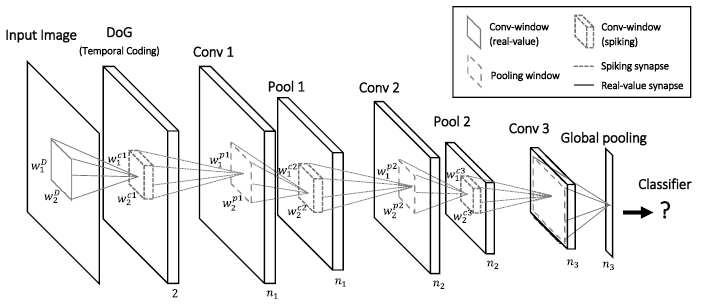
\includegraphics[width=\textwidth]{images/architecture}
	\caption{SDNN architecture}
	\label{fig:architecture}
\end{figure}

\subsection{Temporal coding}

In the very first part of the neural network, the input signal is encoded into temporal-discrete spike events. A Difference of Gaussians (DoG) filter is used to detect the contrasts in the input image and emit a spike, accordingly. The higher the contrast in a certain cell, the more strongly this one is activated in order to fire. The firing time (i.e. the time when the spike is emitted) of a DoG cell is inversely proportional to its activation value. In particular, if an \textit{r} output is obtained in a cell after DoG, its corresponding firing time will be $ \tau = 1/r $. DoG cells are sensitive to both positive and negative contrasts, depending on their two ON-centre and OFF-centre maps and they emit when their activation values exceed a predefined threshold.\\
An example of DoG filter output is shown in figure \ref*{fig:dog}. In this picture, a face and a motor (image categories that compose the learning and training dataset) are encoded into discrete spike events.\\
\begin{figure}[h]
	\centering
	\begin{minipage}[b]{0.48\textwidth}
		
\includegraphics[width=\textwidth]{images/dog_face1}
	\end{minipage}
	\hfill
	\begin{minipage}[b]{0.493\textwidth}
		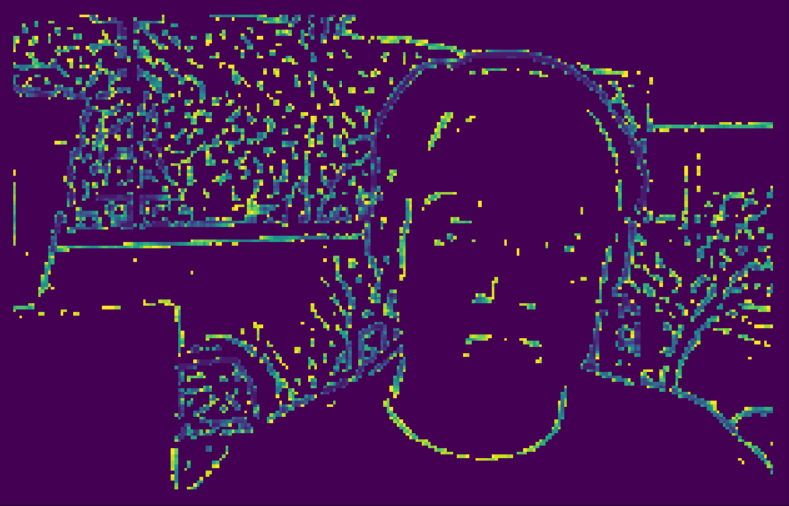
\includegraphics[width=\textwidth]{images/dog_face2}
	\end{minipage}
	\\[0.8em]
	\begin{minipage}[b]{0.498\textwidth}
		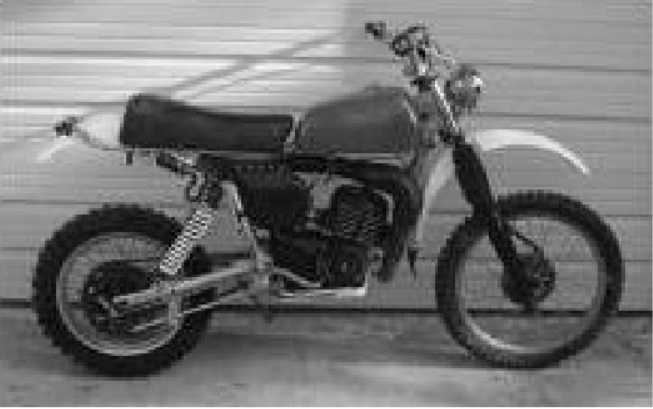
\includegraphics[width=\textwidth]{images/dog_motor1}
	\end{minipage}
	\hfill
	\begin{minipage}[b]{0.482\textwidth}
		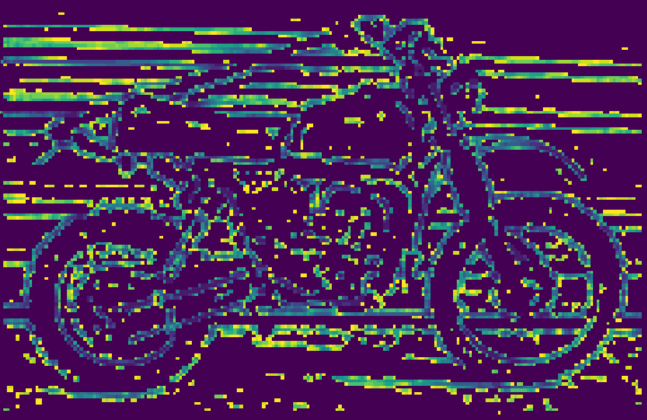
\includegraphics[width=\textwidth]{images/dog_motor2}
	\end{minipage}
	\caption{DoG temporal coding}
	\label{fig:dog}
\end{figure}

\subsection{Convolutional and pooling layers}

A convolutional layer is represented by several neuronal maps, whose role is to detect visual features at different locations. To this extent, the synaptic weights assigned to the same neuronal map will be the same. Each neuron in the convolutional layer generates spikes according to what it receives from the pre-synaptic neurons and when its internal membrane potential reaches a certain threshold. So, at each time step \textit{t}:
\begin{equation*}
	V_{i}(t) = V_{i}(t-1) + \sum_{j}W_{j,i}S_{j}(t-1)
\end{equation*}
the internal potential $ V_{i}(t) $ of the \textit{i-th} convolutional neuron is updated by adding the spike train $ S_{j}(t-1) $ of the \textit{j-th} pre-synaptic neuron, multiplied to the synaptic weight $ W_{j,i} $ between the \textit{j-th} pre-synaptic neuron and \textit{i-th} convolutional neuron. In particular, the potential $ S_{j}(t-1) $ can be equal to 1 if the neuron has fired at previous time, or 0 otherwise. If the neuron potential $ V_{i}(t) $ exceeds the threshold $ V_{th} $, then it emits a spike ($ S_{i}(t) = 1 $) and it resets its potential to zero. After it fires, the neuron can not fire again and it also inhibits other neurons in its same location (but belonging to other neuronal maps). In this way it is easier to detect a visual feature in a certain location.\\
In the pooling layer instead, each neuron performs a max pooling operation over a window in the corresponding neuronal map of the previous layer. Here no learning occurs and, as before, each neuron can emit only one spike. In this phase the visual information is compressed. These convolution-pooling phases are repeated for three times, to handle larger and always more complex data.

\subsection{STDP-based learning}

Spike-timing-dependent plasticity (STDP) is actually a biological process used by brain to modify its own synapses. This same idea has been also used in neural networks, so as to have stronger synapses in case they contribute to the firing of a post-synaptic neuron and weaker synapses if they do not give any contribute to the firing.\\
\begin{figure}[h]
	\centering
	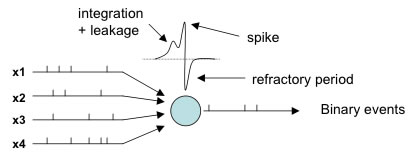
\includegraphics[width=0.75\linewidth]{images/spikes}
	\caption{Contributon to the firing of a post-synaptic neuron}
	\label{fig:spikes}
\end{figure}
This process is easy to understand by looking at figure \ref{fig:spikes}. In this case, four different pre-synaptic neurons are connected to one neuron (the blue one) by synapses. Each of them is characterized by its own firing rate. These spikes are sent forward by the corresponding synapses increasing the membrane potential of the post-synaptic neuron. When this spikes, it is possible to see which pre-synaptic neuron has contributed and its membrane potential is increased. In the same way, the potential of the neurons that have not contributed to the firing of the post-synaptic one, is weakened.\\
As already mentioned, learning occurs only in convolutional layers, so that neurons compete to fire earlier than others and use STDP to learn input patterns. This competition is crucial to encourage neurons of different neuronal maps to learn different features. In this case, STDP is represented as:
\begin{equation*}
	\Delta w_{ij} = \begin{cases}
		a^{+}w_{ij}(1-w_{ij}), & \textit{if }\; t_{j}-t_{i} \leq 0,\\
		a^{-}w_{ij}(1-w_{ij}), & \textit{if }\; t_{j}-t_{i} > 0,
	\end{cases}
\end{equation*}
where \textit{i} and \textit{j} refer to the post-synaptic and pre-synaptic neurons, respectively, $ \Delta w_{ij} $ is the synaptic weight modification and $ a^{+} $ and $ a^{-} $ are the learning rate parameters. The term $ w_{ij}(1-w_{ij}) $ is needed to bound the weight values between 0 and 1. The best choice for the learning rate parameters is with $ a^{+} $ greater than $ a^{-} $, but with small values for both. This, to prevent that neurons learn more than one pattern and/or that do not reach the predefined threshold to fire.\\
It could happen that different neurons fire at the same time, since the time is discrete. In that case, the neuron with the highest potential is selected, since it should define a higher similarity between its learned feature and input pattern.\\
Weights are randomly initiated with mean 0.8 and standard deviation 0.05 and the learning convergence of the \textit{l-th} convolutional layer is represented by:
\begin{equation*}
C_{l} = \sum_{f}\sum_{i}w_{f,i}(1-w_{f,i})/n_{w}
\end{equation*}
where $ n_{w} $ is the total number of synaptic weights in that layer and $ w_{f,i} $ is the \textit{i-th} synaptic weight of the \textit{f-th} feature.

\subsection{Classification}
The third pooling layer is used for the classification, so that each neuron belonging to this layer performs a global max pooling over the corresponding neuronal maps in the previous convolutional layer. Then, one feature can be described by only one output value that is used to train a linear SVM classifier and determining the object's category.
\section{Results}

\section{Conclusions}

\clearpage

\begin{thebibliography}{5}

\bibitem{STPD} 
S. R. Kheradpisheh, M. Ganjtabesh, S. J. Thorpe, and
T. Masquelier, "Stdp-based spiking deep convolutional neural
networks for object recognition," Neural Networks, vol. 99,
pp. 56–67, 2017.

\bibitem{Next-gen}
Spiking Neural Networks, the Next Generation of Machine Learning, https://towardsdatascience.com/spiking-neural-networks-the-next-generation-of-machine-learning-84e167f4eb2b

\bibitem{GitHub}
Spiking-Neural-Network, https://github.com/Shikhargupta/Spiking-Neural-Network
\end{thebibliography}

\end{document}